% !TEX encoding = UTF-8 Unicode
\chapter{准备工作}
\label{chap:chap-3}

\fontsize{12bp}{14.4pt}

\section{局部不可约解析分支}

\begin{defin}
设 $\CC\{t\}, \CC\{x,y\}$ 是所有定义在 $0 \in \CC, (0,0) \in \CC^2$
附近的全纯函数 $z(t), \allowbreak f(x,y)$ 构成的集合, 即
\begin{align*}
    \CC\{t\} &= \bracketcur*{z(t) = \sum_{n=0}^\infty a_nt^n: z(t) \text{ 在
    $0$ 的一个邻域内收敛}},\\
    \CC\{x,y\} &= \bracketcur*{f(x,y) = \sum_{m,n=0}^\infty a_{m,n}x^my^n: f(x,y) \text{ 在
    $(0,0)$ 的一个邻域内收敛}}.
\end{align*}
\end{defin}

显然 $\CC\{t\},\CC\{x,y\}$ 有自然的加法和乘法结构, 因此构成环.
显然 $\CC\{t\}$ 中的单位(可逆元)为 $z(0) \ne 0$ 的全纯函数 $z(t)$,
$\CC\{x,y\}$ 中的单位为 $f(0,0) \ne 0$ 的全纯函数 $f(x,y)$.

\begin{defin}[Weierstrass 多项式]
\label{defin:weier-poly}
如果 $w \in \CC\{x\}[y]\subseteq \CC\{x,y\}$ 满足
\[w(x,y) = y^d + a_{d-1}(x)y^{d-1} + \cdots + a_0(x), \quad a_j(x) \in \CC\{x\},a_j(0) = 0, j = 0,\cdots, d - 1.\]
则称 $w$ 为一个(关于 $y$)的 \textbf{Weierstrass 多项式}.
\end{defin}

\begin{thm}[Weierstrass 预备定理]
\label{thm:Weierstrass-preparation}
设 $f(x,y) \in \CC\{x,y\}$ 满足 $f(0,y)$ 作为 $y$ 的多项式非零,
则在 $(0,0)$ 的一个充分小邻域内, $f(x,y)$ 可以被唯一表示成
\begin{equation}
    \label{eq:weierstrass-preparation}
    f(x,y) = u(x,y)\cdot w(x,y)
\end{equation}
其中 $u(x,y)$ 是 $\CC\{x,y\}$ 中的单位, $w(x,y) \in \CC\{x\}[y]$ 是一个 Weierstrass 多项式.
\end{thm}

\begin{proof}
见 \cite{textbook} 第二章的定理 4.5.
\end{proof}

Weierstrass 预备定理告诉我们, 局部来看(在 $(0,0)$ 的一个充分小邻域内),
$f(x,y)$ 的零点都由 Weierstrass 多项式贡献.

\begin{thm}
\label{thm:UFD}
$\CC\{t\}, \CC\{x\}[y], \CC\{x,y\}$ 都是唯一因子分解整环,
且 $f(x,y) \in \CC\{x\}[y] \subseteq \CC\{x,y\}$ 在小环 $\CC\{x\}[y]$ 中不可约
当且仅当它在大环 $\CC\{x,y\}$ 中不可约.
\end{thm}

\begin{proof}
见 \cite{textbook} 的第二章的推论 4.6.
\end{proof}

设 $z(t) \in \CC\{t\}$, 则 $z(t)$ 的分解情况为:
\begin{equation}
\label{eq:zt}
    z(t) = t^n\cdot h(t), \quad n \in \ZZ_{>0}, h(t) \in \CC\{t\}, h(0) \ne 0.
\end{equation}
也就是说 $\CC\{t\}$ 中的不可约元只有一个 $t$.

设 $f(x,y) \in \CC\{x,y\}$, 则 $f(x,y)$ 的分解情况为:
\begin{equation}
\label{eq:fxy}
    f(x,y) = x^n\cdot u(x,y)\cdot w_1(x,y)\cdots w_d(x,y),
\end{equation}
其中 $n \in \ZZ_{>0}, u(x,y) \in \CC\{x,y\}$ 为可逆元,
$w_j(x,y) \in \CC\{x\}[y], j = 1,\cdots, d$ 为不可约的 Weierstrass 多项式.

现在设 $C$ 是一条不可约代数曲线, 由仿射方程 $f(x,y)$ 给出,
并且不妨假设 $p = (0,0) \in C$, 即 $f(0,0) = 0$.
此时 $f(x,y)$ 虽然在 $\CC[x,y] = \CC[x][y]$ 中不可约,
但是如果我们视 $f(x,y)$ 为 $\CC\{x\}[y]$ 中的元素, 那么它未必是不可约的.
注意, 无论我们视 $f(x,y)$ 为 $\CC\{x\}[y]$ 中的元素还是 $\CC[x][y]$ 中的元素,
它的判别式 $\mathrm{disc}(f)$ 都是一样的,
而因为 $f(x,y)$ 在 $\CC[x][y]$ 中不可约, 所以 $\mathrm{disc}(f) \ne 0$,
这意味着 $f(x,y)$ 在 $\CC\{x\}[y]$ 中的分解也不会含有重因子.
于是 $f(x,y)$ 有形如 \cref{eq:fxy} 的分解(因为
$f(x,y)$ 不可约, 所以 \cref{eq:fxy} 中 $n = 0$):
\begin{equation}
\label{eq:analytic-decomposition}
f(x,y) = u(x,y)\cdot w_1(x,y)\cdots w_s(x,y).
\end{equation}
因为 $u(x,y)$ 为 $\CC\{x,y\}$ 中的可逆元, 即 $u(x,y) \ne 0$,
所以对 $(0,0)$ 的一个充分小的邻域
\[\Delta = \Delta(\rho,\varepsilon) \defeq\{(x,y) \in \CC^2: \abs{x} < \rho, \abs{y} < \varepsilon\},\]
$f(x,y)$ 的零点都由 $w_j(x,y)$ 贡献, 即
\[V(f) \cap \Delta = (V(w_1)\cap \Delta)\cup \cdots \cup (V(w_s)\cap \Delta).\]

\begin{defin}[局部不可约解析分支]
\label{defin:local-irre-component}
称 $V(w_j)\cap \Delta$ 为 $f(x,y)$ 在 $p = (0,0)$ 处的一个\textbf{局部不可约解析分支},
记为 $V_j$.
\end{defin}

现在假设 $w(x,y)$ 是一个不可约的 Weierstrass 多项式,
则 $\mathrm{disc}(w) \eqdef \mathcal{D}(x) \in \CC\{x\}$
是一个关于 $x$ 的在 $0$ 附近有定义的全纯函数.
注意到 $w(0,y) = y^k, k \in \ZZ_{>0}$.
\begin{itemize}
    \ii 若 $k = 1$, 则 $w(0,y)$ 无重根, 此时 $\mathcal{D}(0) \ne 0$;
    \ii 若 $k \ge 2$, 则 $w(0,y)$ 有重根, 此时 $\mathcal{D}(0) = 0$,
    但是 $\mathcal{D}(x)$ 作为一个解析函数, 零点是孤立的.
\end{itemize}
所以无论哪种情况, 我们总能选 $\rho$ 充分小,
使得 $\mathcal{D}(x) \ne 0, \forall\;0 < \abs{x} < \rho$.
同理, 可以选取 $\varepsilon$ 充分小,
使得对任意固定的 $x, \abs{x} < \rho$,
$w(x,y)$ 作为关于 $y$ 的多项式的 $k$ 个零点
$y_i(x), i = 1,\cdots, k$ 都满足模长 $\abs{y_i(x)} < \varepsilon$.
此时可以表
\[w(x,y) = y^k + a_{k-1}(x)y^{k-1} + \cdots + a_0(x) = (y-y_1(x))\cdots (y-y_k(x)).\]
由 $\rho$ 的选取, $\frac{\partial w}{\partial y}(x,y_i(x)) \ne 0$(否则
会推出 $\mathcal{D}(x) = 0$), 于是根据隐函数定理
$y_i(x)$ 在 $x$ 的一个充分小的邻域内全纯,
并且 $y_i(x)$ 能沿单连通区域
\[D \defeq \{x \in \CC: \abs{x} < \rho, x \notin [0,\rho)\} = \Delta(\rho)\setminus [0,\rho)\]
上的任意道路解析延拓.
利用 Riemann monodromy 定理,
我们可以把 $y_i(x)$全纯延拓成 $D$ 上的单值解析函数.
如果我们把 $y_i(x)$ 沿一条从 $[0,\rho)$ 下方并穿过
$[0,\rho)$ 的道路解析延拓,
得到的新的解析函数 $y_i^*(x)$ 依然满足 $w(x,y_i^*(x)) = 0$,
所以 $y_i^*(x)$ 在 $x$ 位于 $[0,\rho)$ 上方的取值
就是某个 $y_j(x), 1 \le j \le k$.
通过这样的方式, 我们得到了 $\{1,\cdots,k\}$ 的一个置换 $\sigma: i \mapsto j$.

\begin{figure}[H]
    \centering
    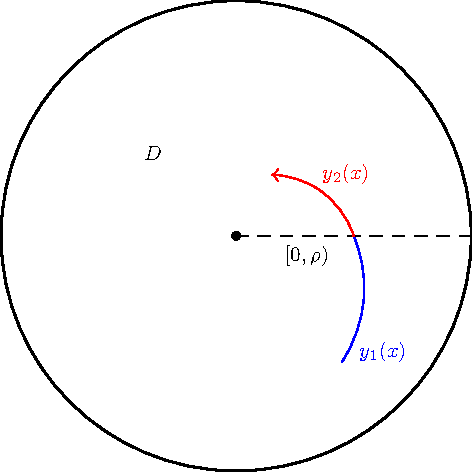
\includegraphics[scale = 0.8]{fig-05.pdf}
    \caption{$y_1(x)$ 沿一条穿过 $[0,\rho)$ 的道路解析延拓变成 $y_2(x)$.}
    \label{fig:analytic-continuation}
\end{figure}

\begin{prop}
\label{prop:irre-criterion}
一个 Weierstrass 多项式 $w(x,y)$ 不可约,
当且仅当 $\sigma$ 就是一个轮换.
\end{prop}

\begin{proof}
\footnote{\cite{textbook}, 第二章引理 5.6}我们先证明: 若 $\sigma$ 是一个轮换, 则
\begin{align*}
f(x,y) &= (y-y_1(x))\cdots (y-y_k(x)) = y^k + b_{k-1}(x)y^{k-1} + \cdots + b_0(x)\\
b_{k-1}(x) &= -(y_1(x) + \cdots + y_k(x))\\
\cdots &= \cdots\\
b_0(x) &= (-1)^ky_1(x)\cdots y_k(x)
\end{align*}
定义的 $f(x,y) \in \CC\{x\}[y]$.
事实上, 因为 $\sigma$ 是轮换,
所以系数 $b_0(x),\cdots, b_{k-1}(x)$ 在沿过 $[0,\rho)$ 的道路解析延拓后不变,
即这些系数都是 $\Delta(\rho)\setminus \{0\}$ 上的全纯函数,
显然它们还都是在 $0$ 的附近有界的(因为 $y_i(x)$ 满足模长 $<\varepsilon$),
这就证明了 $f(x,y) \in \CC\{x\}[y]$.

如果 $\sigma$ 分解成若干个不交轮换的乘积,
则给出了相应的 $w(x,y)$ 分解成若干个 Weierstrass 多项式的乘积,
反之亦然. 所以 $w(x,y)$ 不可约等价于 $\sigma$ 本身就是一个轮换.
\end{proof}

所以, 我们可以不妨假设置换 $\sigma$ 就是 $(12\cdots k)$,
也就是说: $y_i(x)$ 沿绕 $0$ 旋转 $m$ 周的道路延拓后成为 $y_{i+m}(x)$,
特别的 $y_i(x)$ 沿绕 $0$ 旋转 $k$ 周的道路延拓后不变.
在后文里, 如同 \cref{fig:analytic-continuation} 我们总是会假定 $y_i(x)$
沿一条穿过 $[0,\rho)$ 的道路解析延拓后变成 $y_{i+1}(x)$.

\begin{exmp}
$y^2 - x = (y-y_1(x))(y-y_2(x))$,
则每个 $y_i(x)$ 只是 $D$ 上的单值全纯函数,
而不是整个圆盘 $\Delta(\rho)$ 上单值全纯函数.
当我们让 $y_1(x)$ 沿过 $[0,\rho)$ 的道路延拓后,
就变成了 $y_2(x)$.
于是由 \cref{prop:irre-criterion} 知 $y^2 - x$ 在 $\CC\{x\}[y]$ 中不可约.
\end{exmp}

\begin{exmp}
考虑多项式 $f(x,y) = y^2 - x^2 + x^3 \in \CC[x,y] = \CC[x][y] \subseteq \CC\{x\}[y]$.
\begin{itemize}
    \ii $f(x,y)$ 在 $\CC[x,y]$ 中不可约:
    取 $\mathfrak{p} = (x-1)$ 为 $\CC[x]$ 中的素(极大)理想,
    显然 $x^3 - x^2 \notin \mathfrak{p}^2$,
    于是由 Eisenstein 判别法便知 $f(x,y)$ 不可约.
    \ii $f(x,y)$ 在 $\CC\{x\}[y]$ 中可约:
    事实上, $g(x) = x\cdot(1-x)^{\frac{1}{2}}$ 为定义在 $0$ 附近的解析函数(注意
    $(x-1)^{\frac{1}{2}}$ 可以利用广义二项式定理写出幂级数展开),
    满足 $g(x)^2 = x^2 - x^3$, 于是
    \[f(x,y) = (y-g(x))\cdot (y+g(x)).\]
\end{itemize}
当我们把注意力集中在 $x$ 充分小的时候(\cref{fig:local-seeing} 中为 $\abs{x} \le 0.25$),
$f(x,y)$ 近似为两条交于 $(0,0)$ 的曲线的并(这两条曲线分别由 $y = g(x)$ 和 $y = -g(x)$ 决定),
每一条曲线都是 $f(x,y)$ 在 $(0,0)$ 处的一个局部不可约解析分支.
\begin{figure}[H]
    \centering
    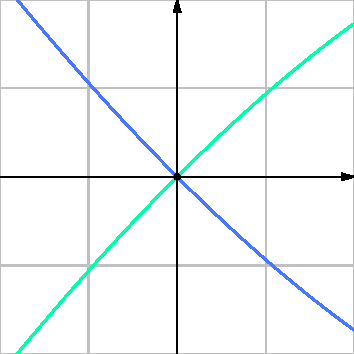
\includegraphics[scale = 1]{fig-04.pdf}
    \caption{局部地看 $f(x,y) = y^2 - x^2 + x^3 = 0$}
    \label{fig:local-seeing}
\end{figure}
\end{exmp}

\begin{rem}
在 $\CC[x,y]$ 中看相当于从整体来观察曲线,
在 $\CC\{x\}[y]$ 中看相当于观察 $\abs{x}$ 充分小时候的曲线,
在 $\CC\{x,y\}$ 中看相当于观察 $\abs{x},\abs{y}$ 同时充分小时候的曲线.
\cref{thm:UFD} 从这个角度来说就是:
曲线在 $\abs{x}$ 充分小时来看(相当于水平聚焦)不可约,
则即使再垂直聚焦也依然不可约.
\end{rem}

\section{正则化定理}

下述正则化定理把代数曲线 $C$ 和 Riemann 面联系了起来.
它可以看成是代数曲线 $C$ 的全纯参数表示,
其中参数取自 Riemann 面的局部坐标表示.
正则化定理的详细证明见 \cite{textbook}.

\begin{thm}[正则化定理]
\label{thm:normalization}
设 $C \subseteq \CP^2$ 为一条不可约代数曲线,
$S$ 是 $C$ 的所有奇点构成的集合,
在全纯同构的意义下,
存在唯一的紧 Riemann 面 $\tilde{C}$ 以及一个全纯映射
\[\sigma: \tilde{C} \to \CP^2\]
满足:
\begin{enumerate}[label=\normalfont(\arabic*)]
    \ii $\sigma(\tilde{C}) = C$;
    \ii 对任意 $p \in C, \sigma^{-1}(p)$ 为 Riemann 面 $\tilde{C}$ 中 $s$ 个不同的点,
    这里 $s$ 是 $p$ 处局部不可约解析分支的个数.
    \ii $\sigma: \tilde{C}\setminus\sigma^{-1}(S) \to C\setminus S$ 是单射.
\end{enumerate}
\end{thm}

\begin{thm}[局部正则化]
\label{thm:local-normalization}
设 $p = (0,0) \in C, \tilde{p} \in \sigma^{-1}(p)$,
正则化映射 $\sigma$ 可局部地表为:
\begin{itemize}
    \ii 若 $p$ 为光滑点, 则 $\frac{\partial f}{\partial x}(x,y)$
    和 $\frac{\partial f}{\partial y}(x,y)$ 不同时为 $0$,
    由隐函数定理知此时 $\sigma$ 为
    \[\sigma: x \mapsto (x,y(x)) \quad \text{or} \quad y \mapsto (x(y),y).\]
    \ii 若 $p$ 为奇点, $V$ 为 $p$ 处的一个局部不可约解析分支, 由 Weierstrass 多项式
    \begin{equation}
    \label{eq:irre-weierstrass}
    w(x,y) = y^l + a_1(x)y^{l-1} + \cdots + a_l(x) = \prod_{\mu=1}^l(y-y_\mu(x))
    \end{equation}
    给出. 则此时 $\sigma$ 为
    \begin{equation}
    \label{eq:local-normalization}
    \sigma: \Delta(\rho^{\frac{1}{l}}) \to V, \quad t\mapsto (t^l, \sigma_y(t)),
    \end{equation}
    \begin{center}
    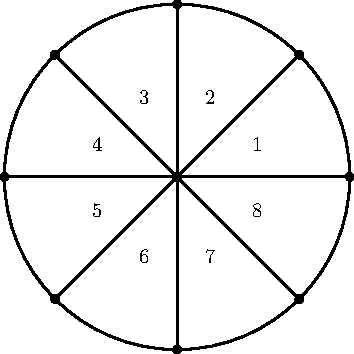
\includegraphics[scale=0.66]{fig-01.pdf}
    \end{center}
    这里我们将 $\Delta(\rho^{\frac{1}{l}})$ 等分为 $l$ 块扇形,
    当 $t$ 位于 $\Delta(\rho^{\frac{1}{l}})$ 中的第 $\mu$ 块扇形时,
    $\sigma(t)$ 的 $y$ 分量 $\sigma_y(t) = y_\mu(t^l)$.
    事实上, $\sigma$ 是 $\Delta(\rho^{\frac{1}{l}})$ 到 $V$ 的全纯双射,
    如果我们视 $V\setminus \{(0,0)\}$ 为一个 Riemann 面,
    则 $\sigma$ 还是 $\Delta(\rho^{\frac{1}{l}})\setminus \{0\}$ 到 $V\setminus \{(0,0)\}$
    的双全纯映射.
\end{itemize}
\end{thm}

\begin{rem}
因为 $y_\mu(x)$ 沿过 $[0,\rho)$ 的道路解析延拓时,
变成了 $y_{\mu + 1}(x)$,
这保证了局部正则化的定义是合理的.
对于 $p$ 是奇点的情形,
我们事实上得到了 $l$ 个不同的局部正则化,
每个局部正则化被 $t$ 位于第一块扇形时,
$\sigma(t)$ 的 $y$ 分量为哪个 $y_\mu(x)$ 唯一决定.
这 $l$ 个局部正则化两两之间只相差一个旋转(逆时针旋转若干次 $\frac{2\pi}{l}$).
\end{rem}

\begin{exmp}[直线的正则化]
\label{exmp:line-normalization}
设 $\ell: \alpha x - \beta y$ 为一条直线,
则它的局部正则化为 $\sigma: t \mapsto (\beta t, \alpha t)$.
\end{exmp}

\begin{exmp}
\label{exmp:non-ordinary-normalization}
代数曲线 $y^2 - x^3 = 0$ 就是一个在 $(0,0)$ 处的局部不可约解析分支(利用
\cref{prop:irre-criterion}),
局部正则化为 $\sigma: t \mapsto (t^2, t^3)$ 或 $t \mapsto (t^2, -t^3)$,
它们的 $y$ 分量差一个逆时针旋转 $\pi$.
\end{exmp}

\begin{exmp}
代数曲线 $y^2 - x^2 + x^3 = 0$ 在 $(0,0)$ 处有两个局部不可约解析分支:
\[y^2 - (x^2 - x^3) = (y - g(x))\cdot (y + g(x)),\]
局部正则化为 $\sigma: t \mapsto (t,g(t))$ 和 $\sigma: t \mapsto (t,-g(t))$.
\end{exmp}

\section{相交数, Bezout 定理}

\begin{defin}[order]
\label{defin:order}
设 $z(t)\in \CC\{t\}, \varphi(x,y) \in \CC\{x,y\}$.
\begin{itemize}
    \ii $z(t)$ 在 $0$ 处有幂级数展开
    \[z(t) = \sum_{n=0}^\infty \alpha_nt^n.\]
    称使得 $\alpha_n \ne 0$ 的最小非负整数 $n$ 为 $z(t)$ (关于 $t$)的 \textbf{order}.
    \ii $\varphi(x,y)$ 可以写成齐次部分的无穷和:
    \[\varphi(x,y) = \sum_{n=1}^\infty \varphi_n(x,y),\]
    其中 $\varphi_n(x,y)$ 为 $\varphi(x,y)$ 的 $n$ 次齐次部分.
    称使得 $\varphi_n(x,y) \ne 0$ 的最小非负整数 $n$
    为 $\varphi(x,y)$ 的 \textbf{order}.
\end{itemize}
\end{defin}

\begin{lem}
\label{lem:order-relation}
设 $w(x,y)$ 是一个由 \cref{eq:irre-weierstrass} 给出的不可约 Weierstrass 多项式,
$\sigma: t \mapsto (t^l, \sigma_y(t))$ 是它的局部正则化.
则我们有 $\sigma_y(t)$ 关于 $t$ 的 order
等于 $a_0(x)$ 关于 $x$ 的 order.
\end{lem}

\begin{proof}
注意事实上我们有 $l$ 个不同的局部正则化 $\sigma^1,\cdots, \sigma^l$,
其中当 $t$ 位于第 $1$ 块扇形时, $(\sigma^\mu)_y(t) = y_\mu(t^l)$.
这 $l$ 个局部正则化两两之间只相差一个旋转,
因而关于 $t$ 有相同的 order. 我们有
\begin{align*}
    \text{order of }(\sigma^1)_y(t) &= \frac{1}{l}\cdot \text{order of }\prod_{\mu=1}^{l}(\sigma^\mu)_y(t)\\
    &=\frac{1}{l}\cdot \text{order of }\prod_{\mu=1}^ly_\mu(t^l)\\
    &=\frac{1}{l}\cdot \text{order of }a_0(t^l)\\
    &=\text{order of }a_0(x).
\end{align*}
\end{proof}

在 \cref{exmp:non-ordinary-normalization} 中,
两个局部正则化分别为 $\sigma: t \mapsto (t^2, t^3)$ 和 $t \mapsto (t^2, -t^3)$,
而 $a_l(x) = a_2(x) = -x^3$, order 都为 $3$.

\begin{defin}[相交数]
\label{defin:intersection-number}
设 $f(x,y), h(x,y) \in \CC\{x\}[y]$ 为 Weierstrass 多项式,
\[V = \{(x,y) \in \CC^2: f(x,y) = 0\}, \quad W = \{(x,y) \in \CC^2: h(x,y) = 0\}\]
相交于 $p$(不妨设为 $p = (0,0)$).
如果 $f(x,y)$ 是不可约的,
设 $V$ 的局部正则化由 $\sigma: t \mapsto (t^l, \sigma_y(t))$ 给出,
定义 $V$ 和 $W$ 在 $p = (0,0)$ 处的\textbf{相交数}为 $h$ 用 $\sigma^*$ 拉回后关于 $t$ 的 order, 即
\[(V\cdot W)_p \defeq \text{order of }\sigma^*(h) = \text{order of }h(t^l,\sigma_y(t)).\]
对一般的由 $f(x,y) \in \CC[x][y]$ 定义的代数曲线,
在 $p = (0,0)$ 处 $V$ 分解为若干个局部不可约解析分支的并:
\[V = m_1V_1 + \cdots + m_lV_l,\]
即 $f(x,y)$ 在 $\CC\{x\}[y]$ 中分解成 $f = f_1^{m_1}\cdots f_l^{m_l}$,
每个 $V_i$ 是 $f_i$ 对应的局部不可约解析分支.
此时我们定义 $V$ 和 $W$ 在 $p$ 点处的相交数为
\[(V\cdot W)_p \defeq \sum_{j=1}^l m_j(V_j\cdot W)_p.\]
最后, 定义 $V$ 和 $W$ 的相交数为
\[(V \cdot W) \defeq \sum_{p \in V\cap W} (V\cdot W)_p.\]
\end{defin}

相交数的定义式中 $V, W$ 的地位是不对等的,
但是如果我们交换 $V, W$ 的位置得到的相交数是一样的(符合我们对相交的直观).

\begin{prop}[相交数的对称性]
$(V\cdot W)_p = (W\cdot V)_p$.
\end{prop}

\begin{proof}
设 $V,W$ 分别由 $f(x,y) = 0, h(x,y) = 0$ 定义, $p = (0,0)$.
我们只需证明结论对 $f(x,y), h(x,y)$ 都是不可约 Weierstrass 多项式时成立.
此时可表
\[f(x,y) = (y-y_1(x))\cdots (y-y_m(x)), \quad h(x,y) = (y-z_1(x))\cdots (y-z_n(x)),\]
其中 $y_i(x), z_j(x), 1 \le i \le m, 1 \le j \le n$
的定义同 \cref{eq:irre-weierstrass},
根据定义我们有
\begin{align*}
    (V\cdot W)_p &= \text{order of }h(t^m, y_i(t^m))\\
    &=\text{order of }\prod_{j=1}^n(y_i(t^m) - z_j(t^m)).
\end{align*}
同理我们有
\[(W\cdot V)_p = \text{order of }\prod_{i=1}^m(z_j(t^n) - y_i(t^n)). \]
但是
\begin{align*}
    \text{order of }\prod_{j=1}^n(y_i(t^m) - z_j(t^m)) &= \text{order of }h(t^m, y_i(t^m))\\
    &=\frac{1}{m}\text{order of }\prod_{i=1}^m h(t^m, y_i(t^m))\\
    &=\frac{1}{m}\text{order of }\prod_{i=1}^m\prod_{j=1}^n (y_i(t^m) - z_j(t^m))\\
    &=\frac{1}{mn}\text{order of }\prod_{i=1}^m\prod_{j=1}^n (y_i(t^{mn}) - z_j(t^{mn})).
\end{align*}
这里第二个等号相当于把 $h$ 用 $m$ 个不同的局部正则化拉回,
它们关于 $t$ 都有相同的 order.
完全类似地可得
\[\text{order of }\prod_{i=1}^m(z_j(t^n) - y_i(t^n))=\frac{1}{mn}\text{order of }\prod_{j=1}^n\prod_{i=1}^m (z_j(t^{mn}) - y_i(t^{mn})).\]
这就证明了 $(V\cdot W)_p = (W\cdot V)_p$.
\end{proof}

\begin{thm}[Bezout]
\label{thm:Bezout}
设 $C, E$ 为两条无公共分支的代数曲线, 即它们的齐次方程(仿射方程)无公共因子,
则有
\[(C\cdot E) = \sum_{p \in C\cap E}(C\cdot E)_p = \deg C \cdot \deg E.\]
\end{thm}

\begin{proof}
见 \cite{textbook} 第二章的定理 7.5.
注意 \cref{prop:line-bezout} 就是 $C,E$ 其中之一为直线的情形.
\end{proof}

现在设 $\varphi(x,y) \in \CC\{x\}[y]$ order 为 $n$,
\[\varphi(x,y) = \varphi_n(x,y) + \varphi_{n+1}(x,y) + \cdots.\]
因为 $\CC$ 是代数闭域, 它的 $n$ 次齐次部分 $\varphi_n(x,y)$ 可以分解成 $n$ 条直线的乘积:
\[\varphi_n(x,y) = (\alpha_1x - \beta_1y)\cdots (\alpha_nx - \beta_ny).\]
我们称这 $n$ 条直线为 $\varphi(x,y)$ 在 $(0,0)$ 处的切线.

\begin{prop}[相切的刻画]
\label{prop:tangent-chara}
设 $\ell: \alpha x - \beta y$ 是一条直线,
$\varphi(x,y) \in \CC\{x\}[y]$. 以下陈述等价:
\begin{enumerate}[label=\normalfont(\arabic*)]
    \ii $\ell$ 与 $\varphi(x,y)$ 相切.
    \ii $\ell$ 是 $\varphi(x,y)$ 的 $n$ 次齐次部分的因子.
    \ii $\text{order of }\varphi(\beta t,\alpha t) > n$.
    \ii $(\ell\cdot V(\varphi))_{(0,0)} > n$.
\end{enumerate}
\end{prop}

设 $C$ 是由仿射方程 $f(x,y)$ 给出的不可约代数曲线,
$f(x,y)$ 在 $\CC\{x\}[y]$ 中可进一步分解成 \cref{eq:analytic-decomposition}.
注意到我们有
\begin{equation}
\label{eq:order-sum-relation}
\sum_{j=1}^s \text{order of $w_j(x,y)$} = \text{order of $f(x,y)$}.
\end{equation}
而 order of $f(x,y)$ 正是 $p = (0,0)$ 的重数, 记为 $k$.
若我们表
\[w_j(x,y) = y^{l_j} + a_{l_j-1}^j(x)y^{l_j - 1} + \cdots + a_0^j(x),\]
则有 $l_j \ge n_j$, 以及 $k_j\defeq$ order of $a_0^j(x) \ge n_j$,
这里 $n_j \defeq \text{order of }w_j(x,y)$.
如果我们一开始就已经作了适当的旋转变换,
使得 $f(x,y)$ 在 $(0,0)$ 处的切线都不是 $x = 0$,
即 $y^k$ 出现在 $f(x,y)$ 的 $k$ 次齐次项中,
则此时必有 $l_j = n_j$(否则, 会推出 $y^k$ 的系数为 $0$).

\begin{prop}
\label{prop:only-one-tangent}
对每个局部不可约解析分支 $w_j(x,y)$, 在不计重数的意义下
有且只有一条直线 $\ell: \alpha x - \beta y$ 与它相切.
\end{prop}

\begin{proof}
设 $\sigma: t \mapsto (t^{l_j}, \sigma_y(t))$ 为 $w_j(x,y)$ 的局部正则化,
由 \cref{lem:order-relation} 知 $\sigma_y(t)$ 的 order 为 $k_j$, 于是可以表
\[\sigma_y(t) = \sum_{n = l_j}^\infty \alpha_nt^n,\quad \alpha_{k_j} \ne 0.\]
由相交数的对称性,
我们有 $\ell$ 与 $w_j(x,y)$ 相切
当且仅当 $(\ell \cdot V_j)_{(0,0)} > n_j = l_j$, 而
\[(\ell\cdot V_j)_{(0,0)} = \text{order of }\paren*{\alpha t^{l_j} - \beta \sum_{n=l_j}^\infty \alpha_nt^n}.\]
由此可见, $(\ell\cdot V_j)_{(0,0)} > l_j$ 当且仅当 $\alpha - \beta\alpha_{l_j} = 0$,
这就说明了与局部不可约解析分支 $w_j(x,y)$ 相切的直线有且只有
$y - \alpha_{l_j}x$ 这一条.
\end{proof}

\begin{cor}
\label{cor:ordinary}
设 $C$ 是一条不可约代数曲线, $p \in C$ 为 $k$ 重奇点,
则 $C$ 在 $p$ 处的局部不可约解析分支个数 $\le k$,
等号当 $p$ 为普通奇点时成立.
\end{cor}

\begin{proof}
第一个结论由 $w_j(0,0) = 0 \implies n_j \ge 1$, 再利用 \cref{eq:order-sum-relation} 推出.
当 $p$ 为普通奇点时,
在不计重数的意义下我们有 $k$ 条不同的切线.
另一方面, 注意到 $\ell$ 与 $C$ 在 $p$ 处相切,
当且仅当 $\ell$ 与某个局部不可约解析分支 $w_j(x,y)$ 相切,
于是由 \cref{prop:only-one-tangent} 知,
在不计重数的意义下, $C$ 在 $p$ 处至多有 $s$ 条不同的切线,
这推出 $k \le s$, 所以此时只能是 $k = s$.
\end{proof}

\begin{cor}
\label{cor:ordinary-normalization}
设 $p = (0,0)$ 是代数曲线 $C$ 的普通 $k$ 重奇点,
则 $C$ 在 $p$ 处的局部正则化可表为
\[\sigma: t \mapsto (t,y(t)) \quad \text{or} \quad \sigma: t \mapsto (x(t),t),\]
这里 $x(t), y(t) \in \CC\{t\}$.
\end{cor}

\begin{proof}
当 $p$ 是普通奇点时, 我们有 $k = s$,
以及 $n_j = 1, \forall\; j$.
注意 $n_j = 1$ 可以推出要么 $l_j = 1$, 要么 $k_j = 1$,
所以局部正则化 $\tau$
或者形如 $t \mapsto (t,y(t)), y(t) \in \CC\{t\}$,
或者形如 $t \mapsto (t^{l_j}, y(t))$, 其中 $y(t) \in \CC\{t\}$ 且 $y'(0) \ne 0$.
对于后者, 因为 $y'(0) \ne 0$, 利用反函数定理可以表 $t = \psi(y), \psi(y) \in \CC\{y\}$,
再命 $\sigma \defeq \tau\circ \psi$,
则 $\sigma(y) = \tau(t) = (\psi(y)^{l_j}, y) \eqdef (x(y), y)$.
\end{proof}

\begin{prop}
\label{prop:singularity-intersection-number}
设 $p = (0,0)$ 在代数曲线
\[V = \{(x,y) \in \CC^2:f(x,y) = 0\},\quad W = \{(x,y) \in \CC^2: h(x,y) = 0\}\]
中重数分别为 $k, m$, 则 $(V\cdot W)_p \ge km$.
\end{prop}

\begin{proof}
因为 $p = (0,0)$ 的重数分别为 $m, k$, 我们有
\[f(x,y) = f_k(x,y) + f_{k+1}(x,y) + \cdots, \quad h(x,y) = h_{m}(x,y) + h_{m+1}(x,y) + \cdots.\]
其中 $f_k(x,y), h_m(x,y)$ 分别为 $f,h$ 的 $k,m$ 次齐次部分.
$f(x,y)$ 可以进一步分解成同 \cref{eq:analytic-decomposition},
对每个局部不可约解析分支 $w_j(x,y)$, 我们有 $l_j \ge n_j, k_j \ge n_j$,
并且由 \cref{lem:order-relation} 知 $\sigma_y(t)$ 的 order $= k_j \ge n_j$,
这里 $\sigma$ 是 $w_j(x,y)$ 在 $p$ 处的局部正则化.
于是 order of $\sigma^*(h) = h(t^{l_j},\sigma_y(t)) \ge n_j\cdot m$,
故 $(V\cdot W)_p = \sum_{j=1}^s n_j\cdot m = km$.
\end{proof}

